% -----------------------------------------------------------------------------
%                     Universidade Federal de São João del-Rei - UFSJ
% -----------------------------------------------------------------------------
%                Modelo de Trabalho Acadêmico conforme as normas da ABNT
%         (Tese de Doutorado, Dissertação de Mestrado ou Projeto de Qualificação)
%
%                            Autor: Gabriel Victor Costa Pereira
%
%                          Créditos a Cristiano Fraga G. Nunes (CEFET)
%                   
% -----------------------------------------------------------------------------

% Utiliza um modelo para impressão apenas no anverso
\documentclass[oneside]{UFSJ}

% -----------------------------------------------------------------------------
%                           Pacotes Utilizados
% -----------------------------------------------------------------------------
% Codificação do documento
\usepackage[utf8]{inputenc}         

% Seleção de fonte e estilo de formatação
\usepackage[T1]{fontenc}            
\usepackage{palatino}                % Fonte 'Palatino' (clone)
%\usepackage[charter]{mathdesign}    % Fonte 'Charter BT'
%\usepackage{newtxtext, newtxmath}   % Fonte 'Times New Roman' (clone)
%\usepackage{lmodern}                % Fonte 'Computer Modern'
%\usepackage[scaled]{helvet}         % Fonte 'Arial' (clone)
%\renewcommand*\familydefault{\sfdefault}

% Melhorias na formatação e layout do documento
\usepackage{microtype}              % Aperfeiçoamento da justificação do texto
\usepackage{indentfirst}            % Recuo do primeiro parágrafo de cada seção

% Funcionalidades avançadas para tabelas
\usepackage{booktabs}               % Linhas horizontais de qualidade nas tabelas
\usepackage{makecell}               % Criação de células com múltiplas linhas ou colunas
\usepackage{multirow, multicol}     % Layout de múltiplas linhas ou colunas
\usepackage{color, colortbl}        % Uso de cores nas tabelas

% Gráficos e imagens
\usepackage{graphicx}               % Inclusão de gráficos e imagens

% Exibição e formatação de texto
\usepackage{verbatim}               % Exibição de texto tal como escrito
\usepackage{xfrac}                  % Frações de maneira compacta

% Expressões matemáticas
\usepackage{amsmath}                % Operações matemáticas avançadas
\usepackage{amsfonts}               % Fontes matemáticas
\usepackage{latexsym}               % Símbolos adicionais de matemática
\usepackage{icomma}                 % Vírgulas nas expressões matemáticas
\usepackage{subeqnarray}            % Subenumeração de equações

% -----------------------------------------------------------------------------
% Configurações gerais
% -----------------------------------------------------------------------------

% Define o tamanho do recuo do parágrafo
\setlength{\parindent}{1.25cm}

% Define o espaçamento entre um parágrafo e outro
\setlength{\parskip}{0.0cm}

% Define as cores utilizadas no documento
\definecolor{blue_link}{RGB}{0,80,128}

% Define as palavras-chave nos metadados do PDF
\hypersetup{pdfkeywords={%
    Palavra-chave 1, Palavra-chave 2, Palavra-chave 3, Palavra-chave 4.
}}

% -----------------------------------------------------------------------------
% Inclui os arquivos do trabalho acadêmico
% -----------------------------------------------------------------------------

% Inclui o arquivo que contém os dados do trabalho acadêmico
% -----------------------------------------------------------------------------
% Dados do trabalho acadêmico
% -----------------------------------------------------------------------------

\titulo{Quando a Casa Cai}
%\title{Title in English}
\subtitulo{Uma Análise Computacional da Casa dos Três Porquinhos}
\autor{Lobo Mau}
\local{São João del-Rei, MG}
\data{Dezembro de 202X} 

% -----------------------------------------------------------------------------
% Tipo de documento acadêmico
% Escolha apenas uma das categorias a seguir:
% - Tese (destinada ao nível de Doutorado)
% - Dissertação (aplicável ao nível de Mestrado)
% - Trabalho de Conclusão de Curso (referente à graduação)
% -----------------------------------------------------------------------------

\projeto{Trabalho de Conclusão de Curso}

% -----------------------------------------------------------------------------
% Identificação do título acadêmico
% Utilize apenas uma das opções listadas:
% - Doutor (referente a Doutorado)
% - Mestre (para Mestrado)
% - Bacharel (para cursos de Graduação)
% -----------------------------------------------------------------------------

\tituloAcademico{Bacharel}

% -----------------------------------------------------------------------------
% Dados da instituição
% -----------------------------------------------------------------------------

\instituicao{UNIVERSIDADE FEDERAL DE SÃO JOÃO DEL-REI}
\programa{CURSO DE ENGENHERIA MECÂNICA}

% -----------------------------------------------------------------------------
% Definição da área de concentração e linha de pesquisa
% Observação: Especifique o nome da área de concentração e a linha de pesquisa
% correspondente ao programa de Pós-graduação ao qual este trabalho pertence. 
% Caso a natureza do trabalho seja Trabalho de Conclusão de Curso, mantenha
% ambos os campos em branco.
% -----------------------------------------------------------------------------

\areaconcentracao{}
\linhapesquisa{}
\logoinstituicao{4cm}{figuras/logo_vazado}

% -----------------------------------------------------------------------------
% Orientador(es)
% -----------------------------------------------------------------------------

\orientador{Prof. D.Sc. João Silva}
%\orientador[Orientadora:]{Nome da orientadora}
\instOrientador{Universidade Federal de São João del-Rei}

\coorientador{Prof. D.Sc. Marcos Silva}
%\coorientador[Coorientadora:]{Nome da coorientadora}
\instCoorientador{Universidade Federal de São João del-Rei}

% -----------------------------------------------------------------------------
% Folha de Rosto
% -----------------------------------------------------------------------------

% Trabalho de Conclusão de Curso
\preambulo{{\imprimirprojeto} apresentado ao Curso de Engenharia Mecânica da Universidade Federal de São João del-Rei, como requisito parcial para a obtenção do título de {\imprimirtituloAcademico} em Engenharia Mecânica.}



% Início do documento
\begin{document}

\pretextual
\imprimircapa
\imprimirfolhaderosto*{}           

% -----------------------------------------------------------------------------
% Folha de aprovação
% -----------------------------------------------------------------------------

\makeatletter
\begin{folhadeaprovacao}

    % Imprime o nome do autor
    \begin{center}
        \normalfont\large\scshape\textbf\imprimirautor
    \end{center}

    % Espaço vertical
    \vspace*{\stretch{2}}

    % Imprime o título do trabalho
    \begin{center}
        \ABNTEXchapterfont\LARGE\scshape\SingleSpacing{%
            \imprimirtitulo%
            \abntex@ifnotempty{\imprimirsubtitulo}{%
                {:\\}{\Large\imprimirsubtitulo}}%
        }
    \end{center}

    % Espaço vertical
    \vspace*{\stretch{0.5}}

    % Imprime o preâmbulo
    \abntex@ifnotempty{\imprimirpreambulo}{%
        \hspace{.3\textwidth}
        \hyphenpenalty=10000\hbadness=10000%
        \begin{minipage}{.6\textwidth}
            \imprimirpreambulo
        \end{minipage}
    }

    % Espaço vertical
    \vspace*{\stretch{0.5}}

    \begin{center}
        Trabalho Aprovado. \imprimirlocal, XX de Dezembro de 202X: 
    \end{center}

    % Imprime os nomes dos membros
    \abntex@ifnotempty{\imprimirorientador}{\assinatura{\imprimirorientador \\ \imprimirinstOrientador}}
    \abntex@ifnotempty{\imprimircoorientador}{\assinatura{\imprimircoorientador \\ \imprimirinstCoorientador}}
    \assinatura{Prof. D.Sc. Antônio Silva  \\ Universidade Federal de São João del-Rei}

    % Espaço vertical
    \vspace*{\stretch{0.5}}

    % Imprime local e data
    \begin{center}
        \normalfont{\imprimirlocal}\\
        \normalfont{\imprimirdata}
    \end{center}

\end{folhadeaprovacao}
\makeatother



% -----------------------------------------------------------------------------
% Dedicatória
% -----------------------------------------------------------------------------

\begin{dedicatoria}

    Dedicatória.

\end{dedicatoria}
          % Dedicatória
% -----------------------------------------------------------------------------
% Agradecimentos
% -----------------------------------------------------------------------------

\begin{agradecimentos}

\colorbox{yellow}{COPIADO TEMPLATE PFC II.}

Ao Prof. Dr. Orientador, braço amigo de todas as etapas deste trabalho.

A minha família, pela confiança e motivação.

Aos amigos e colegas, pela força e pela vibração em relação a  esta jornada.

Aos professores e colegas de Curso, pois juntos trilhamos uma etapa importante de nossas vidas.

Aos profissionais entrevistados, pela concessão de informações valiosas para a realização deste estudo.

A todos que, com boa intenção, colaboraram para a realização e finalização deste trabalho.

Ao professor coordenador de TCC que sempre me incentivou a estudar mais para dar maior qualidade à minha monografia.


\end{agradecimentos}
       % Agradecimentos
% -----------------------------------------------------------------------------
% Epígrafe
% -----------------------------------------------------------------------------

\begin{epigrafe}

    \textit{``A primeira casa dos porquinhos era feita de palha, mas eles aprenderam que um bom planejamento é a chave para a resistência.''}
    (GPT, Chat)

\end{epigrafe}
             % Epígrafe
% -----------------------------------------------------------------------------
% Resumo
% -----------------------------------------------------------------------------

\begin{resumo}

\colorbox{yellow}{COPIADO TEMPLATE PFC II.}

O resumo deve ser apresentado em parágrafo único e justificado. Deverá conter no máximo 1800 caracteres contando-se os espaçamentos. O resumo deverá conter, obrigatoriamente: (1) Introdução, (2) Objetivos, (3) Amostra, (4) Procedimentos Experimentais; (5) Estatística (quando houver); (6) Resultados; (7) Discussão; e, (8) Conclusão. Todavia, não utilize tópicos colocando em negrito ou sublinhado cada um destes elementos mencionados acima. Utilize uma estrutura de texto de resumo em texto corrido que, por si só, seja capaz de caracterizar cada um dos elementos acima descritos como obrigatórios no resumo. Utilize linguagem objetiva. Nenhum dos tópicos do resumo deverá exceder em seu volume. A ‘Introdução’ deverá ser breve, assim como o ‘Objetivos’ (recomendo no máximo 2 linhas para cada tópico). Transcreva apenas as informações mais importantes nos métodos. Não é necessário detalhar tudo o que foi realizado nos ‘Procedimentos Experimentais’. A caracterização da ‘Amostra’ deve ser sucinta, apenas para dar uma noção de algumas de suas particularidades. Nos ‘Procedimentos Experimentais’, apenas relate as informações que consigam caracterizar os métodos utilizados. Nos ‘Resultados’, indique apenas os dados mais interessantes (que demonstraram significância estatística, por exemplo) e que foram discutidos posteriormente na ‘Discussão’. A ‘Discussão’ é a parte mais importante de um trabalho científico. Nela,, deverá ser apresentada a explicação para os resultados apresentados no estudo. Na ‘Discussão’ também serão verificadas as inferências do estudo sobre os resultados. Por fim, a ‘Conclusão’ deverá ser apresentada com possíveis implicações do estudo, generalizações dos resultados e sugestões de futuros estudos.

    \par\vspace{\baselineskip}

    \textbf{Palavras-chave}: De três a cinco palavras chaves que expressem o conteúdo e tema do trabalho. As palavras-chave devem ser separadas por ponto e vírgula (;).
\end{resumo}
               % Resumo
% -----------------------------------------------------------------------------
% Abstract
% -----------------------------------------------------------------------------

\begin{resumo}[ABSTRACT]

\colorbox{yellow}{COPIADO TEMPLATE PFC II.}

O abstract deverá ser uma tradução fiel da versão em português do estudo. O abstract é obrigatório para o TCC. Não serão aceitas traduções realizadas por meios eletrônicos sem que haja devida revisão por profissional qualificado. Para tanto, após concluir a versão final do resumo do TCC, procure um professor de Inglês habilitado ou uma pessoa com conhecimento em língua inglesa avançada para revisar seu ABSTRACT. Pois, serão poucos os professores orientadores que possuirão domínio sobre a língua inglesa. Ou seja, a maioria dos orientadores não se responsabilizará por fazer esta tradução do RESUMO para o ABSTRACT. Desta forma, fica de inteira responsabilidade do aluno encontrar algum meio de realizar a devida tradução do RESUMO para o ABSTRACT. Reforço que o ABSTRACT é parte avaliada na banca de defesa final como item necessário para aprovação. 

    \par\vspace{\baselineskip}

    \textbf{Keywords}: De três a cinco palavras chaves que expressem o conteúdo e tema do trabalho. As palavras-chave devem ser separadas por ponto e vírgula (;). Devem-se utilizar as palavras em inglês referentes às traduções das palavras-chave utilizadas no RESUMO em português.


\end{resumo}

             % Abstract

\imprimirlistafiguras                                   % Lista de figuras
\imprimirlistatabelas                                   % Lista de tabelas
\imprimirlistaquadros                                   % Lista de quadros
\imprimirlistaalgoritmos                                % Lista de algoritmos

% -----------------------------------------------------------------------------
% Lista de Siglas
% -----------------------------------------------------------------------------

\begin{siglas}
    \item[ABNT] Associação Brasileira de Normas Técnicas
    \item[IGL] In-game leader
    \item[MDS] Meu Deus
    \item[NT] Nice Try
    \item[TKV] Trem Ki Voa
\end{siglas}

% -----------------------------------------------------------------------------
% Edite a lista acima para definir as siglas utilizadas neste trabalho.
% -----------------------------------------------------------------------------
                   % Lista de siglas
% -----------------------------------------------------------------------------
% Lista de Símbolos
% -----------------------------------------------------------------------------

\begin{simbolos}
    \item[$\alpha$]   Letra grega Alfa
    \item[$\beta$]    Letra grega Beta
    \item[$\gamma$]   Letra grega Gama
    \item[$\delta$]   Letra grega Delta
    \item[$\epsilon$] Letra grega Épsilon
    \item[$\zeta$]    Letra grega Zeta
    \item[$\eta$]     Letra grega Eta
    \item[$\theta$]   Letra grega Teta
    \item[$\iota$]    Letra grega Iota
    \item[$\kappa$]   Letra grega Kappa
    \item[$\lambda$]  Letra grega Lambda
    \item[$\mu$]      Letra grega Mi
    \item[$\nu$]      Letra grega Ni
    \item[$\xi$]      Letra grega Xi
    \item[$o$]        Letra grega Ômicron
    \item[$\pi$]      Letra grega Pi
    \item[$\rho$]     Letra grega Rô
    \item[$\sigma$]   Letra grega Sigma
    \item[$\tau$]     Letra grega Tau
    \item[$\upsilon$] Letra grega Upsilon
    \item[$\phi$]     Letra grega Fi
    \item[$\chi$]     Letra grega Chi
    \item[$\psi$]     Letra grega Psi
    \item[$\omega$]   Letra grega Ômega
\end{simbolos}

% -----------------------------------------------------------------------------
% Edite a lista acima para definir os símbolos utilizados neste trabalho.
% -----------------------------------------------------------------------------
                 % Lista de símbolos
\imprimirsumario                                        % Sumário

\textual % Define o estilo de página para os elementos textuais

% -----------------------------------------------------------------------------
% Introdução
% -----------------------------------------------------------------------------

\chapter{INTRODUÇÃO} % Letra Maiúscula
\label{introducao}

\colorbox{yellow}{COPIADO TEMPLATE PFC II.}

Na introdução é exposto o tema central do trabalho e seu contexto em nossa sociedade e/ou curso, relacionando, caso exista, com o objeto foco do estudo (estudo de caso, caso seja este o método de pesquisa), seguido por: objetivo geral (com a definição do problema), objetivos específicos (itens secundários para se atender o objetivo geral).

Na introdução deve ser explicitado o problema de pesquisa de forma explícita, por exemplo com uma questão problema; ou de forma implícita, a partir da contextualização e dissertação acerca do tema. É comum o uso de citações da literatura para contextualizar o tema de pesquisa e o problema. É comum também conter uma justificativa sobre a importância do tema ser pesquisado, sempre considerando a literatura como referência para tal.

Para facilitar a padronização dos textos de PFC, são adotadas as seguintes regras de formatação do texto: Fonte: Times New Roman; Tamanho 12 para texto e 16 para títulos. Tamanho 10, para citações diretas longas e legendas (de Figuras e Tabelas); Espaço entre linhas e parágrafos: espaçamento entre linhas 1,5, e 0 pontos após o término de um parágrafo. Tamanho de folha A4, com margens superior e esquerda 3 cm, e direita e inferior 2 cm. Usar recuo no início de parágrafos. Os parágrafos devem estar justificados à direita e a esquerda. Usar como referência a formatação do presente texto.

A língua oficial para todos os trabalhos é a língua portuguesa. Caso o aluno opte pelo uso da língua inglesa para fins de publicação, o orientador deve consentir. Palavras escritas em idioma diferente da língua portuguesa devem estar em itálico (caso o português seja a língua oficial do trabalho). Todos os títulos de seções devem estar alinhados à esquerda e em negrito. Títulos das seções primárias devem ter todas as letras maiúsculas. Usar as dimensões de folha A4. Margens do texto: esquerda e superior: 3 cm. Direita e inferior: 2 cm.
Todas as páginas deverão ser numeradas, com exceção da capa e das páginas de anexo e apêndices (anexos e apêndices são opcionais). A numeração deve ser em algarismos arábicos, no canto inferior direito da folha.

O curso de Engenharia de Mecânica da UFSJ entende o PFC como sendo um dos passos finais para a obtenção do grau de bacharel em Engenharia Mecânica. Nesse sentido, o PFC visa avaliar a capacidade do graduando de desenvolver um trabalho acadêmico sob a orientação de um docente que atua no curso de Engenharia Mecânica em tema de interesse do discente.

\section{OBJETIVOS} % Letra Maiúscula

Na seção objetivo, são apresentados os objetivos geral e específicos para a obtenção dos resultados pretendidos. O objetivo geral é apresentado em uma única frase, de forma clara e concisa, além do resultado final pretendido ao término de seu artigo. Os objetivos específicos são objetivos secundários que devem ser realizados para alcançar o objetivo geral (principal), sendo estes elencados em tópicos, contendo um verbo no infinitivo, por tópico.

               % Introdução
% -----------------------------------------------------------------------------
% Revisão da Literatura
% -----------------------------------------------------------------------------

\chapter{REVISÃO DE LITERATURA} % Letra Maiúscula
\label{revisao}

Esta seção é a parte do trabalho onde o graduando apresentará o embasamento necessário para o desenvolvimento do trabalho. É o item que contém a maioria das citações, descrevendo o estado da arte do tema abordado. Sugere-se na maioria dos casos o uso de citações indiretas. As citações diretas devem ser usadas somente se as exatas palavras do autor forem extremamente importantes. Geralmente a revisão contém citações de métodos/abordagens propostas para resolver o problema em estudo; de objetos de estudo (problema) nos quais o método foi aplicado, de como foram medidos os resultados; e de conceitos e definições caso sejam importantes para o desenvolvimento da pesquisa. Equações também podem ser usadas para quantificar as definições.       % Revisão de Literatura
% -----------------------------------------------------------------------------
% Metodologia
% -----------------------------------------------------------------------------

\chapter{METODOLOGIA} % Letra Maiúscula
\label{metodologia}

Na metodologia o acadêmico deve definir quais etapas seguiu para desenvolvimento do seu PFC. Ele deve também descrever seu objeto de estudo. Nesta seção é interessante definir qual foi o método de pesquisa, como estudo de caso, pesquisa-ação, etc. Basta descrever as etapas definidas no trabalho, ferramentas, métodos e instrumentos utilizados para coleta de dados, além de programas e pacotes computacionais utilizados para análises.              % Metodologia
% -----------------------------------------------------------------------------
% Resultados
% -----------------------------------------------------------------------------

\chapter{RESULTADOS} % Letra Maiúscula
\label{resultados}

Consiste na descrição detalhada dos resultados obtidos ou esperados com a execução da metodologia proposta. Estes resultados têm de ser mensuráveis com números, e de preferência com valores monetários (o quanto se espera de ganho ou redução de perda de recursos) ou dados estatísticos no caso de revisão da literatura.

São utilizados três elementos não textuais: Figuras, Tabelas e Equações. A indicação ou chamada para as figuras, tabelas e equações deve ser feita no texto, antes destes aparecerem e pela numeração. Os termos Figura, Tabela e Equação sempre são escritos com a inicial maiúscula quando fizerem referência a um elemento não textual presente no trabalho. Por convenção, são utilizadas sequências crescentes em algarismos arábicos para numerar Figuras, Tabelas e Equações, uma sequência para cada elemento não textual. Não use expressões como “Figura abaixo”, “Tabela acima”, “Equação a seguir” e similares.

Utilize figuras com boa resolução. Uma figura ilegível atrapalha mais do que ajuda. Tabelas nunca devem ser inseridas como Figuras. As legendas de figuras e tabelas são dispostas acima destas e centralizadas. As referências (fontes) das tabelas e figuras são apresentadas abaixo das mesmas, a exemplo da Figura 1 e Tabela 1.                % Resultados
% -----------------------------------------------------------------------------
% Conclusão
% -----------------------------------------------------------------------------

\chapter{CONCLUSÃO} % Letra Maiúscula
\label{conclusao}

Na conclusão os objetivos do trabalho devem ser retomados. Sugere-se comparar os resultados obtidos com os objetivos geral e específicos. Pode-se complementar com a opinião pessoal sobre os pontos positivos e negativos a respeito do desenvolvimento do trabalho. Sugere-se a proposição de possíveis trabalhos futuros a serem elaborados considerando as limitações do trabalho finalizado.               % Resultados

\postextual % Define o estilo de página para os elementos pós-textuais

\imprimirreferencias{referencias.bib}         % Referências
% -----------------------------------------------------------------------------
% Apêndices
% -----------------------------------------------------------------------------

\begin{apendicesenv}
    \partapendices

    % -------------------------------------------------------------------------
    % Primeiro apêndice
    % -------------------------------------------------------------------------

    \chapter{APÊNDICE DE INSTRUÇÃO}
    \label{apendice_a}

    É importante lembrar que a distinção entre apêndice e anexo está relacionada à autoria do material ou texto incluído.

    Se o conteúdo suplementar ou complementar for de sua própria autoria, ele deve ser classificado como apêndice. Por outro lado, se a autoria for de outra pessoa, o material deve ser apresentado como anexo.

    Se necessário, você pode incluir outros anexos em seu trabalho acadêmico. Para isso, basta copiar e colar este trecho no mesmo documento.

    Organize seus anexos de forma que cada um contenha apenas um tipo específico de conteúdo. Isso tornará a leitura e a compreensão mais fáceis para o leitor.

    % -------------------------------------------------------------------------
    % Novo apêndice
    % -------------------------------------------------------------------------

    \chapter{ILUSTRAÇÕES}
    \label{ilustracoes}

    A seguir, apresenta-se a maneira de incluir ilustrações no corpo do texto. De acordo com as normas, as figuras, tabelas, quadros, equações, algoritmos, diagramas, entre outros, são considerados tipos específicos de ilustrações.

    \section{TABELAS}
    \label{tabelas}

    Exemplo de tabela:

    \begin{table}[htb!]
\centering
\caption{Condições de contorno para velocidade e pressão.}
\label{tab:ccopenfoam}
\begin{tabular}{lcc}
\toprule

Condição         & Velocidade         & Pressão       \\ \midrule
Entrada          & fixedValue         & zeroGradient  \\
Saída            & zeroGradient       & fixedValue(0) \\
Paredes laterais & slip               & zeroGradient  \\
Rotor            & movingWallVelocity & zeroGradient  \\ \bottomrule
\end{tabular}
\fonte{Gabriel}
\end{table}

    \section{FIGURAS}

    A \autoref{fig_1} é automaticamente incluída na lista de figuras. Já a \autoref{fig_figura_exemplo2} apresenta um exemplo de figura que contém múltiplas imagens.

    \begin{figure}[!htb]
        \centering
        \caption{Domínio computacional empregado nas simulações.}
        \label{fig_1}
        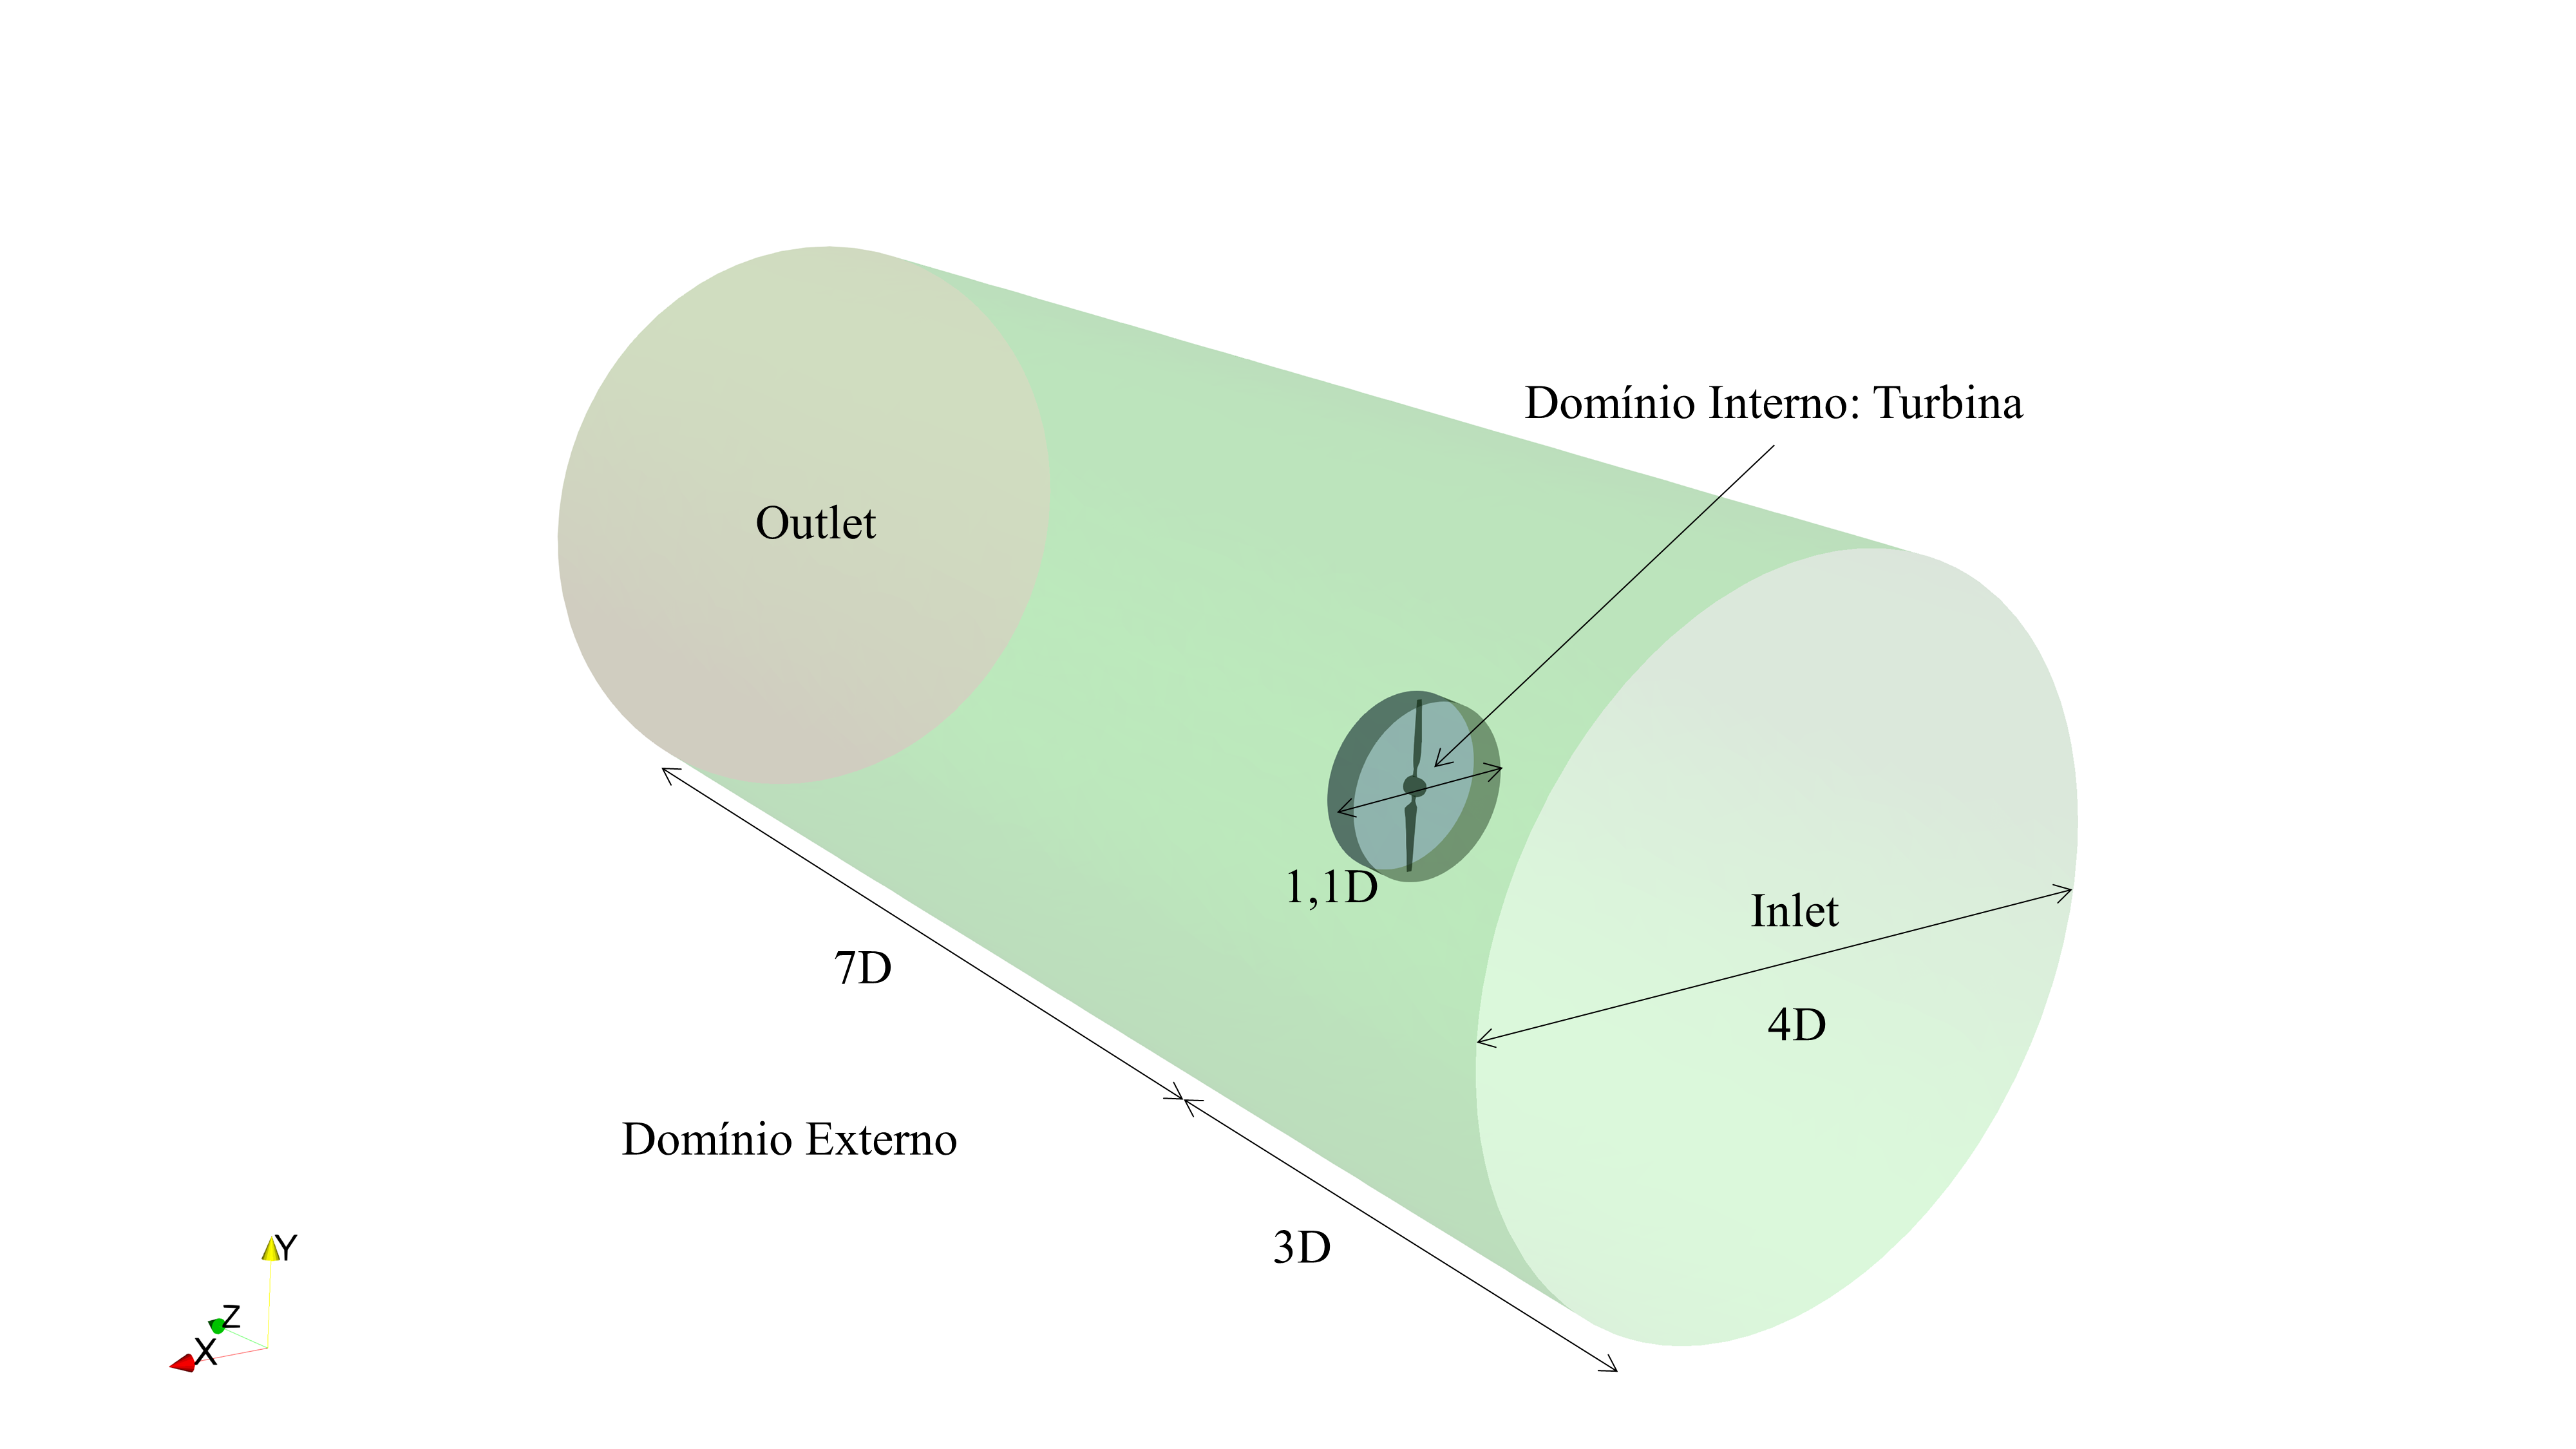
\includegraphics[width=0.75\textwidth]{figuras/domain.png}
        \fonte{Gabriel}
    \end{figure}

    \begin{figure}[!htb]
        \centering
        \caption{Exemplo.}
        \label{fig_figura_exemplo2}
        \subtop[][Exemplo.]{%
            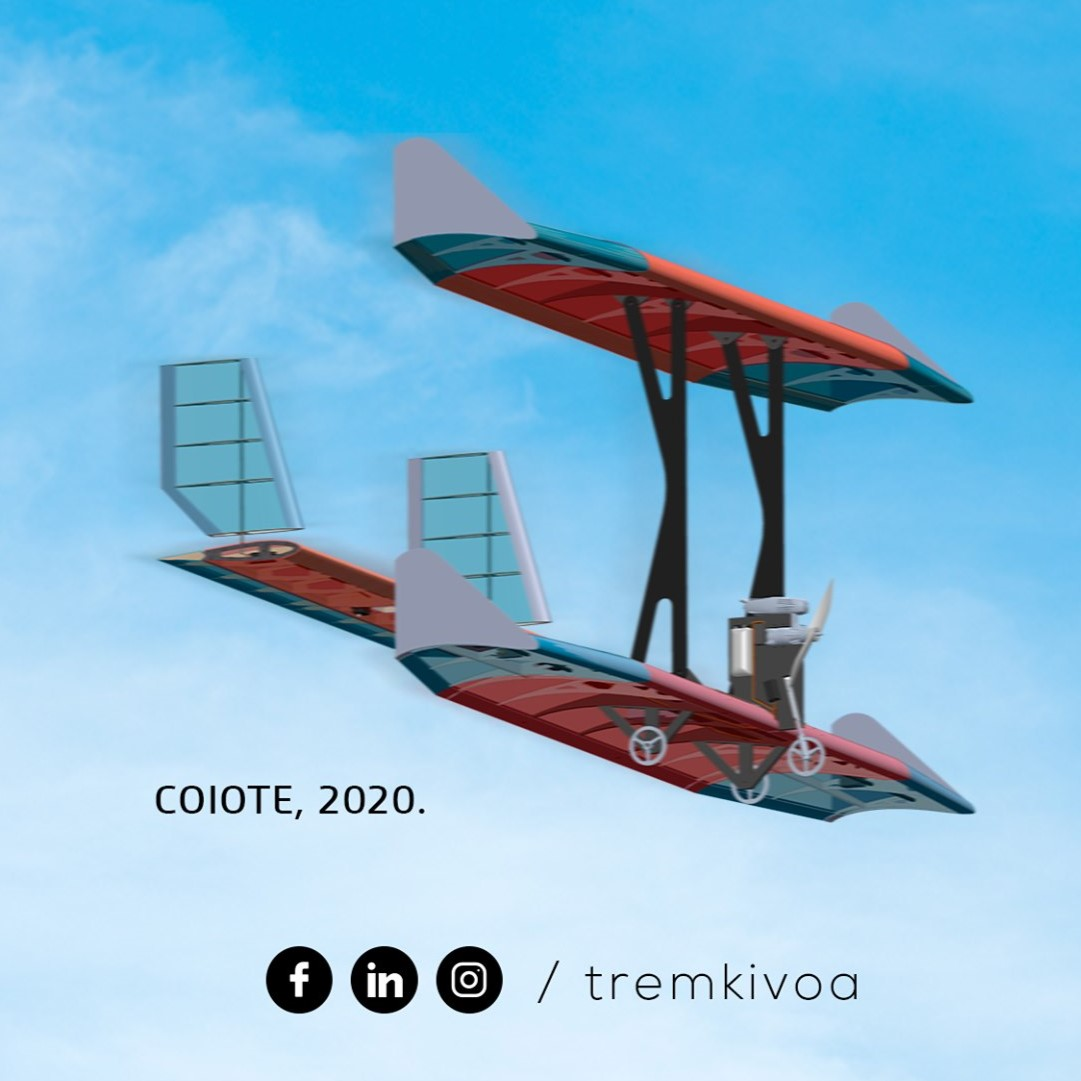
\includegraphics[scale=0.2]{figuras/tkv.jpg}%
        }\hspace{2ex}
        \subtop[][Exemplo.]{%
            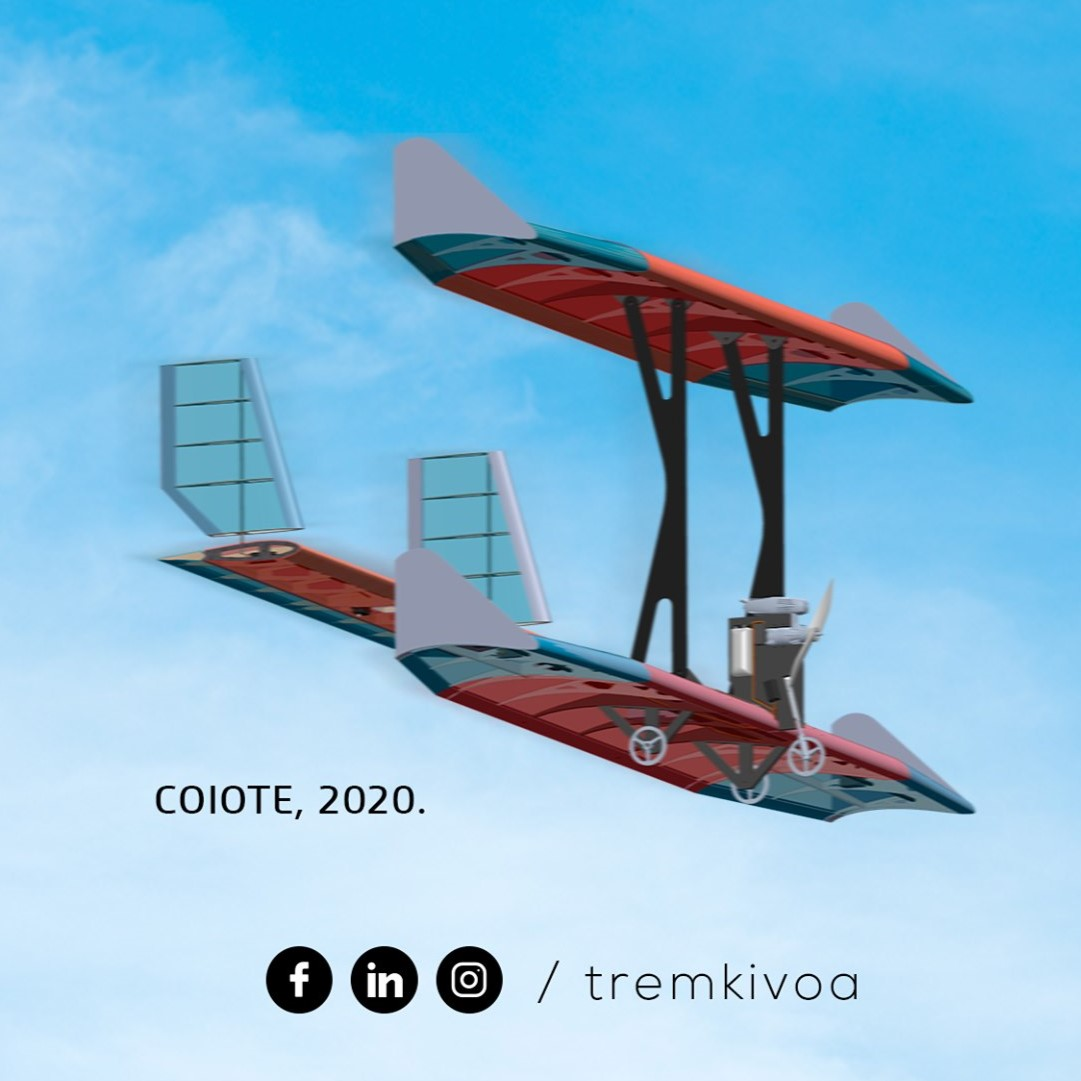
\includegraphics[scale=0.2]{figuras/tkv.jpg}%
        }\hspace{2ex}
        \subtop[][Exemplo.]{%
            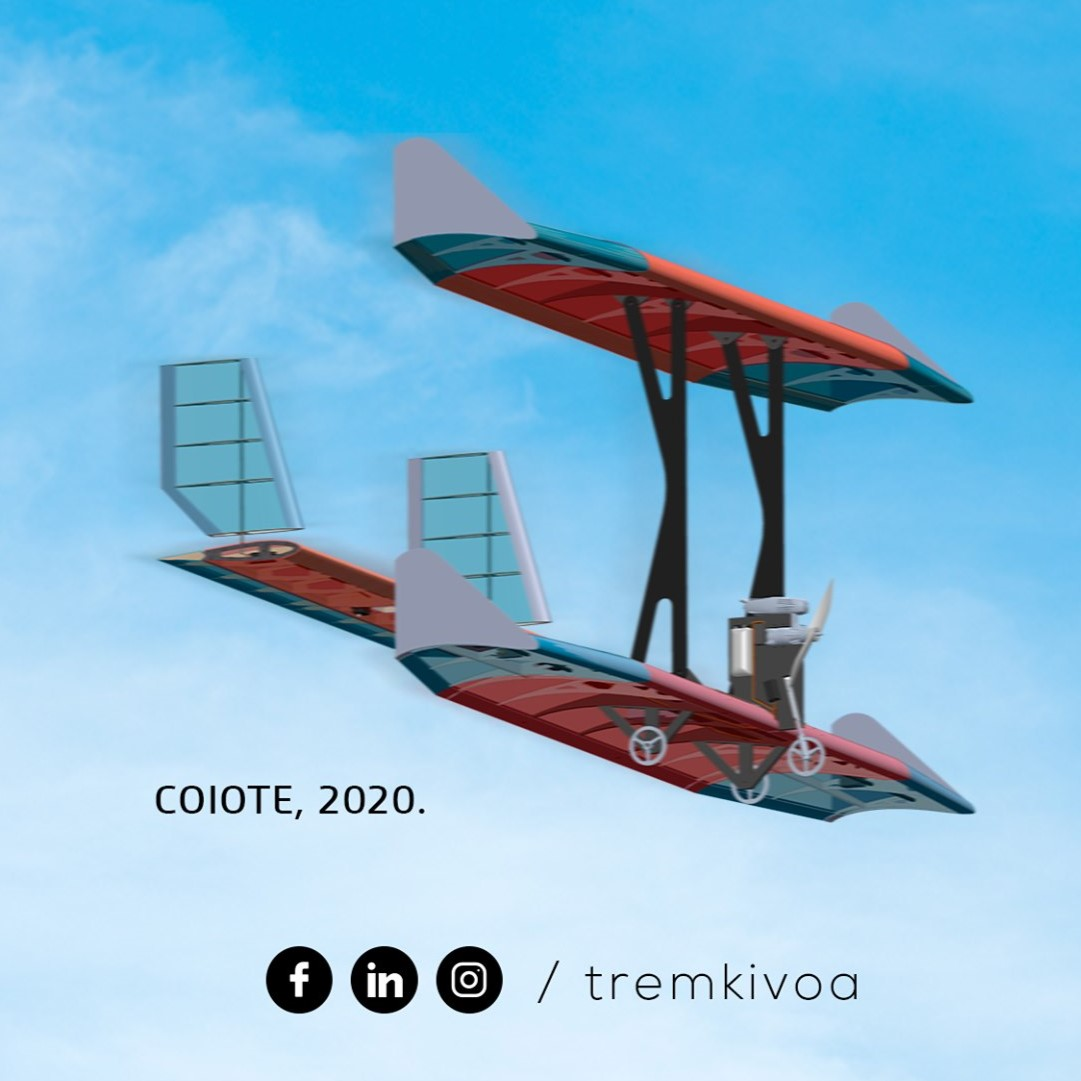
\includegraphics[scale=0.2]{figuras/tkv.jpg}%
        }
    \end{figure}

    \section{EQUAÇÕES}
    \label{equacoes}

   Para o modelo SST $k/\omega$, a energia turbulenta de fluxo livre e a taxa de dissipação da energia turbulenta foram calculadas pelas expressões:

    \begin{equation}
    k = \frac{3}{2} (U_\infty \cdot I)^{2}
    \label{eq41}
    \end{equation}
    e

    \begin{equation}
    \omega = \frac{k^{0.5}}{C_{\mu}^{0.25} L}, \\
    \epsilon =\frac{C_{\mu}^{0.75}k^{1.5}}{L},
    \label{eq42}
    \end{equation}
    onde $I$ = 5\% é a intensidade de turbulência e $L$ a escala de comprimento.

    \section{ALGORITMOS}
    \label{algoritmos}

    Os \index{algoritmos} algoritmos devem ser feitos segundo o \autoref{alg_verificacao_primo}:

    \begin{algorithm}
    \caption{Algoritmo para verificação de número primo (gerado pelo ChatGPT)}
    \label{alg_verificacao_primo}

    \KwIn{um número inteiro $n \geq 2$}
    \KwOut{verdadeiro se $n$ é primo, falso caso contrário}
    \If{$n = 2$}{ 
        \KwRet{verdadeiro} \\
    }
    \If{$n \mod 2 = 0$}{ 
        \KwRet{falso} \\
    }
    $i \leftarrow 3$ \\
    \While{$i \leq \sqrt{n}$}{
        \If{$n \mod i = 0$}{
            \KwRet{falso} \\
        }
        $i \leftarrow i + 2$ \\
    }
    \KwRet{verdadeiro} \\
    
    \end{algorithm}


\end{apendicesenv}
            % Apêndices
% -----------------------------------------------------------------------------
% Anexos
% -----------------------------------------------------------------------------

\begin{anexosenv}
    \partanexos

    % -------------------------------------------------------------------------
    % Primeiro anexo
    % -------------------------------------------------------------------------

    \chapter{ANEXO DE INSTRUÇÃO}
    \label{anexo_a}

    É importante lembrar que a distinção entre apêndice e anexo está relacionada à autoria do material ou texto incluído.

    Se o conteúdo suplementar ou complementar for de sua própria autoria, ele deve ser classificado como apêndice. Por outro lado, se a autoria for de outra pessoa, o material deve ser apresentado como anexo.

    Se necessário, você pode incluir outros anexos em seu trabalho acadêmico. Para isso, basta copiar e colar este trecho no mesmo documento.

    Organize seus anexos de forma que cada um contenha apenas um tipo específico de conteúdo. Isso tornará a leitura e a compreensão mais fáceis para o leitor.
    
\end{anexosenv}               % Anexos
\printindex                                   % Índice remissivo

\end{document}
